\section{Antenna Design 1 -- Monopole}
In this section, the antenna from Section~\ref{sec:techsol1_monopole} will be simulated in pratice use with an user. The antenna positions are shown in Figure~\ref{fig:sol1_monoant_positions}.

\begin{figure}[htbp]
    \centering
    \begin{subfigure}[b]{0.24\linewidth}
        \centering 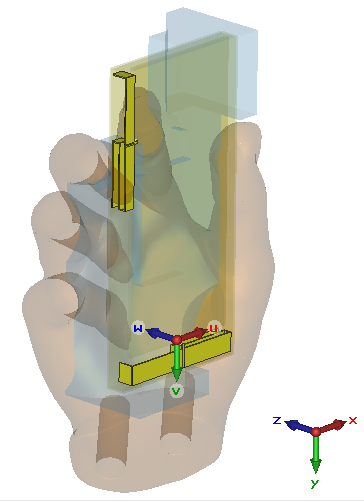
\includegraphics[width=\linewidth,height=4cm,keepaspectratio]{img/tech_sol/monopole/data_mode/3d_data_mode.PNG}
        \caption{Data mode.}
    \end{subfigure}
    \begin{subfigure}[b]{0.24\linewidth}
        \centering 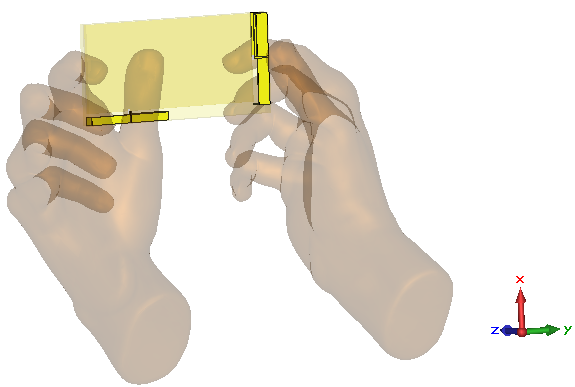
\includegraphics[width=\linewidth,height=4cm,keepaspectratio]{img/tech_sol/monopole/play_mode/3d_play_mode.PNG}
        \caption{Play mode.}
    \end{subfigure}
    \begin{subfigure}[b]{0.24\linewidth}
        \centering 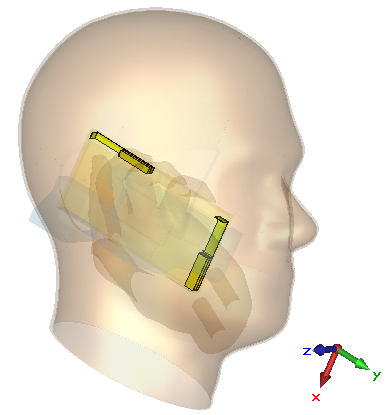
\includegraphics[width=\linewidth,height=4cm,keepaspectratio]{img/tech_sol/monopole/talk_mode/3d_talk_mode.PNG}
        \caption{Talk mode.}
    \end{subfigure}
    \begin{subfigure}[b]{0.24\linewidth}
        \centering 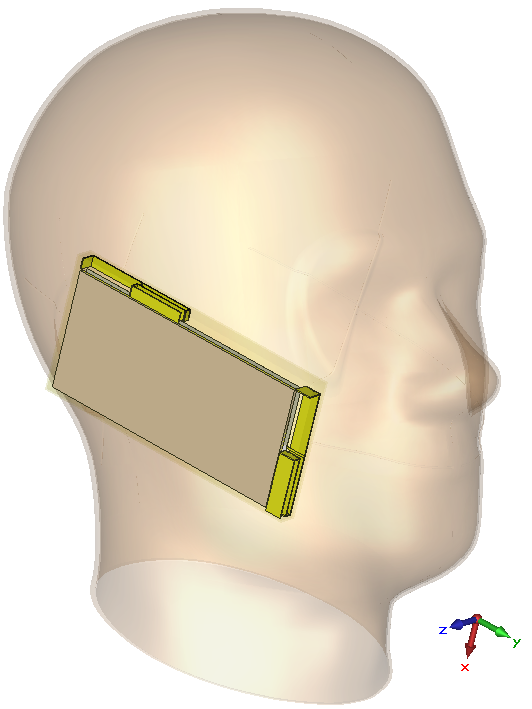
\includegraphics[width=\linewidth,height=4cm,keepaspectratio]{img/tech_sol/monopole/sar/3d_sar.PNG}
        \caption{SAR.}
    \end{subfigure}
    \caption{MIMO monopole antenna position for each user effect simulation.}
    \label{fig:sol1_monoant_positions}
\end{figure}

\FloatBarrier
\subsection{Data Mode}
%S-parameter
The S-parameter sweeps for the data mode, can be seen on Figure \ref{fig:sparam_mono_data_mode}. The highest obtainable bandwidth for both antennas is found from the S-parameter sweep and is listed in Table \ref{tab:bw_sol1data}. The top antenna covers the required bandwidth in both the low and high band. However, as seen in the Table \ref{tab:bw_sol1data} the side antenna only covers the bandwidth in the high band and the low band needs additional tuning to fulfill the bandwidth requirements. The S-parameter sweeps \ref{fig:sparam_mono_data_mode} also shows the $S_{21}$ isolation loss. The highest notable isolation loss is within the low band, at \SI{10}{dB} and \SI{8}{dB} for the top and side antenna respectively.       

%Correlation
The correlation between the top and side antenna can be seen in Figure \ref{fig:corr_sol1_data}. The correlation is plotted sweeping the tunable capacitors of each antenna, while the other antenna is fixed with a tunable at \SI{0.3}{pF}. The correlation for the top and side antenna is below 0.5 for both the low and high band as desired.

%Efficiency
The efficiency in data mode for both antennas, can be seen in Figure \ref{fig:eff_sol1_data}. The efficiency is plotted for each sweep of the tunable capacitors. Comparing the efficiency in data mode with the free space efficiency, the data mode generally decreases over the entire spectrum for both antennas. The different sweep modes of the tunable capacitor shows most significant efficiency drop in the low band with a maximum drop of \SI{-8}{dB} for the top antenna and \SI{-9}{dB} for the side antenna. Both antennas covers the free space requirement of \SI{-3}{dB} efficiency within the frequency band \SI{1710}{MHz} to \SI{2200}{MHz}. 

\begin{figure}[htbp]
    \centering
    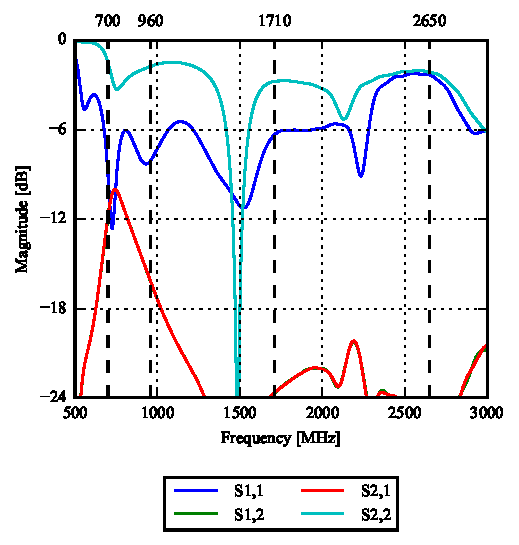
\includegraphics{img/tech_sol/monopole/data_mode/sparam_data.pdf}
    \caption{Monopole antenna in data mode. S-parameters with both tuning capacitors fixed at \SI{0.3}{pF}.}
    \label{fig:mono_sparam_data}
\end{figure}

\begin{table}[htbp]
  \centering
  \begin{tabular}{|l|l|r|r|r|}
    \hline
    Antenna & Band & Start [MHz] & Stop [MHz] & Bandwidth [MHz] \\
    \hline
    Top     & Low  &  677  & 1065  & 388 \\
    Side    & Low  &  700  & 710  & 10  \\
    \hline
    Top     & High &  1183 &  2127  & 944 \\
    Side    & High & 1765 &  2120 & 355 \\
    \hline
  \end{tabular}
  \caption{Monopole antenna in data mode. Maximum bandwidth obtained in the low and high band for the top and the side antenna, respectively.}    
  \label{tab:bw_sol1data}
\end{table}

\begin{figure}[htbp]
   \begin{subfigure}[b]{0.49\linewidth}
        \centering
        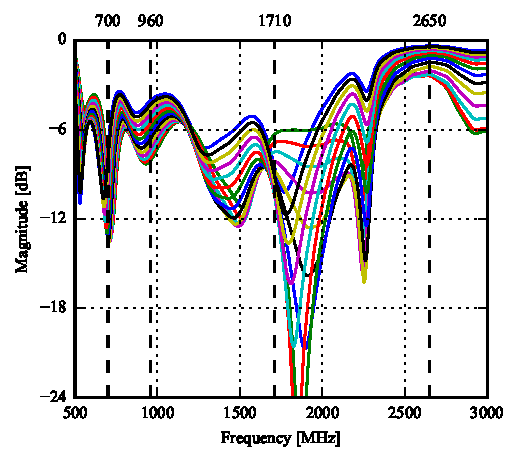
\includegraphics{img/tech_sol/monopole/data_mode/s11}
        \caption{$S_{11}$, sweeping $C_1$ and fixing $C_2$.}
    \end{subfigure}
    \hfill
    \begin{subfigure}[b]{0.49\linewidth}
        \centering
        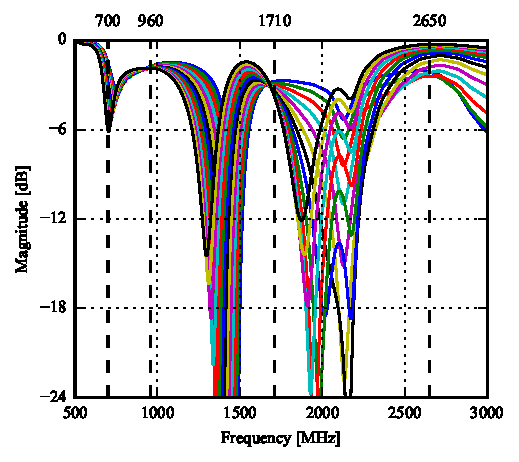
\includegraphics{img/tech_sol/monopole/data_mode/s22}
        \caption{$S_{22}$, sweeping $C_2$ and fixing $C_1$.}
    \end{subfigure}
~
    \begin{subfigure}[b]{0.49\linewidth}
        \centering
        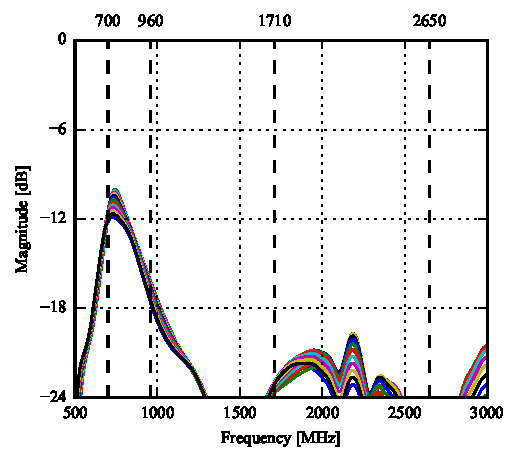
\includegraphics{img/tech_sol/monopole/data_mode/s21_s11}
        \caption{$S_{21}$, sweeping $C_1$ and fixing $C_2$.}
    \end{subfigure}
    \hfill
    \begin{subfigure}[b]{0.49\linewidth}
        \centering
        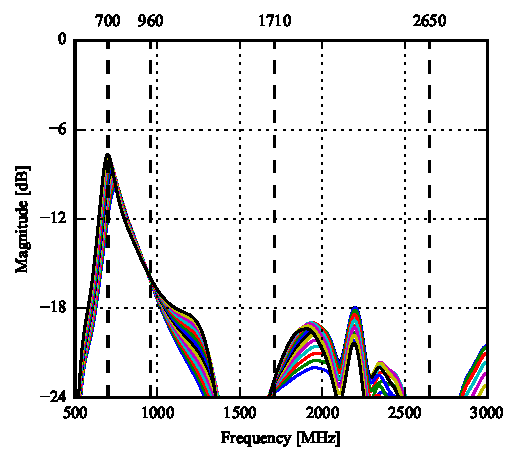
\includegraphics{img/tech_sol/monopole/data_mode/s21_s22}
        \caption{$S_{21}$, sweeping $C_2$ and fixing $C_1$.}
    \end{subfigure}
    \caption{S-parameter sweep in data mode for tuning the shunt capacitor of each antenna, $C_1$ and $C_2$ for port 1 and 2, respectively. Port 1 is the top antenna and port 2 is the side antenna.}
    \label{fig:sparam_mono_data_mode}
\end{figure}

% Correlation
\begin{figure}[htbp]
    \centering
    \begin{subfigure}{0.49\linewidth}
        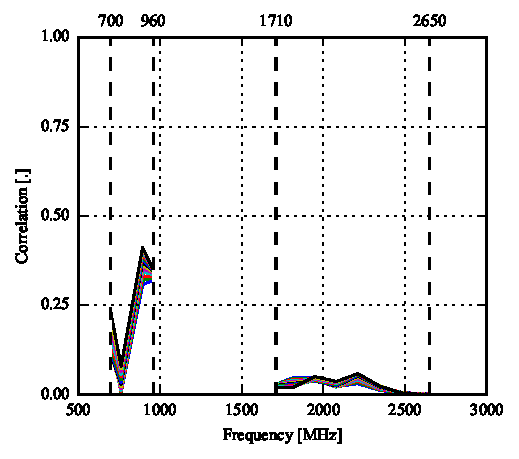
\includegraphics{img/tech_sol/monopole/data_mode/s11_corr}
        \caption{Sweeping $C_1$ and fixing $C_2$.}
    \end{subfigure}
    \hfill
    \begin{subfigure}{0.49\linewidth}
        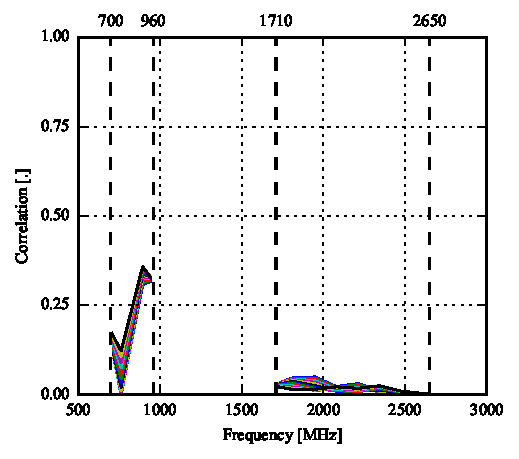
\includegraphics{img/tech_sol/monopole/data_mode/s22_corr}
        \caption{Sweeping $C_2$ and fixing $C_1$.}
    \end{subfigure}
    \caption{Monopole antenna in data mode. Correlation between antennas when sweeping tuning capacitors. Here, $C_1$ and $C_2$ are the tuning capacitor for the top and side antenna, respectively.}
    \label{fig:corr_sol1_data}
\end{figure}

% Efficiency
\begin{figure}[htbp]
    \centering
    \begin{subfigure}{0.49\linewidth}
        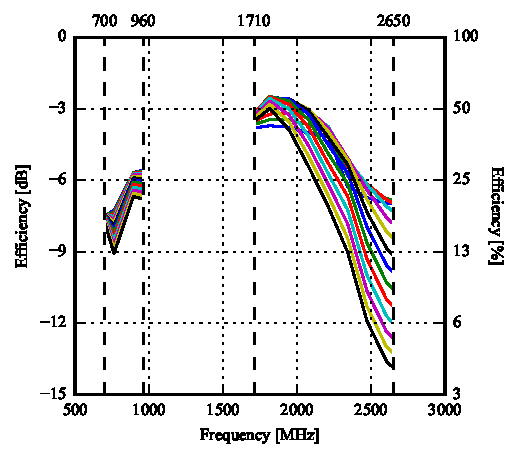
\includegraphics{img/tech_sol/monopole/data_mode/efficiency-ac1-csh1}
        \caption{Sweeping $C_1$ and fixing $C_2$.}
    \end{subfigure}
    \hfill
    \begin{subfigure}{0.49\linewidth}
        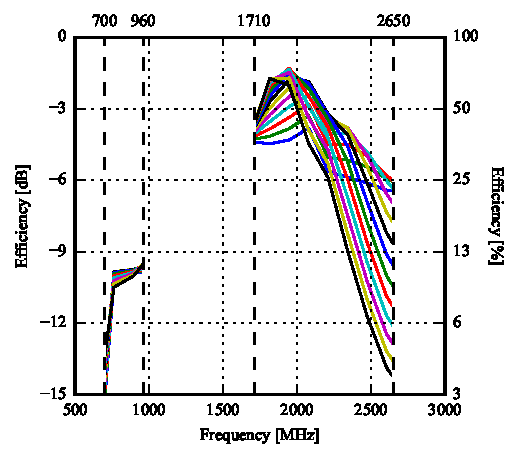
\includegraphics{img/tech_sol/monopole/data_mode/efficiency-ac2-csh2}
        \caption{Sweeping $C_2$ and fixing $C_1$.}
    \end{subfigure}
    \caption{Monopole antenna in data mode. Efficiency for each antenna when sweeping the tunable capacitors. Here, $C_1$ and $C_2$ are the tuning capacitor for the top and side antenna, respectively.}
    \label{fig:eff_sol1_data}
\end{figure}

\FloatBarrier
\subsection{Play Mode}
%S-parameter
The S-parameter sweeps for the data mode, can be seen on Figure \ref{fig:sparam_mono_play_mode}. The highest obtainable bandwidth for both antennas is found from the S-parameter sweep and is listed in Table \ref{tab:bw_sol1play}. The top antenna covers the required bandwidth in the low band but lacks \SI{87}{MHz} in the high band. The side antenna does not fulfill any of the bandwidth requirements and will need additional tuning. The S-parameter sweeps \ref{fig:sparam_mono_play_mode} also shows the $S_{21}$ isolation loss. The highest notable isolation loss is within the low band, at \SI{12}{dB} and \SI{10}{dB} for the top and side antenna respectively.       

%Correlation
The correlation between the top and side antenna can be seen in Figure \ref{fig:corr_sol1_play}. The correlation is plotted sweeping the tunable capacitors of each antenna, while the other antenna is fixed with a tunable at \SI{0.3}{pF}. The correlation for the top and side exceeds the required correlation limit with 0.1 in the low band from \SI{700}{MHz} to \SI{880}{MHz}.

%Efficiency
The efficiency in play mode for both antennas, can be seen in Figure \ref{fig:eff_sol1_play}. The efficiency is plotted for each sweep of the tunable capacitors. Comparing the efficiency in play mode with the free space efficiency, the data mode generally decreases over the entire spectrum for both antennas. The different sweep modes of the tunable capacitor shows most significant efficiency drop in the low band. However comparing the individual sweep modes the highest efficiency drop for the top antenna is within the high band at \SI{2500}{MHz} and within the low band  at \SI{960}{MHz}for the side antenna. The top antenna has a maximum drop of \SI{-10}{dB} for the top antenna and for the side antenna the efficiency drop is greater than \SI{-14}{dB}.
Both antennas has the highest efficiency within the frequency band of \SI{1800}{MHz} to \SI{2200}{MHz} with an efficiency of approx \SI{-5}{dB}. 
The simulation results are as expected compared to the data mode, as the play mode introduces body losses from two hands. 

\begin{figure}[htbp]
    \centering
    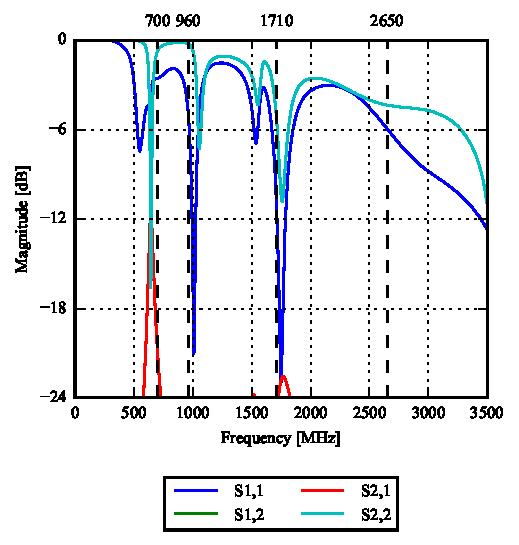
\includegraphics{img/tech_sol/monopole/play_mode/sparams_play.pdf}
    \caption{Monopole antenna in play mode. S-parameters with both tuning capacitors fixed at \SI{0.3}{pF}.}
    \label{fig:mono_play_sparam_data}
\end{figure}

\begin{table}[htbp]
    \centering
    \begin{tabular}{|l|l|r|r|r|}
      \hline
      Antenna & Band & Start [MHz] & Stop [MHz] & Bandwidth [MHz] \\
      \hline
      Top     & Low  & 920 & 1000 &  80 \\
      Side    & Low  & 1010 & 1060 & 50 \\
      \hline
      Top     & High & 1420 & 2053 & 633 \\
      Side    & High & 1635 & 2180 & 545 \\
      \hline
    \end{tabular}
    \caption{Monopole antenna in play mode. Maximum bandwidth obtained in the low and high band for the top and the side antenna, respectively.}    \label{tab:bw_sol1play}
  \end{table}

  \begin{figure}[htbp]
    \begin{subfigure}[b]{0.49\linewidth}
      \centering
      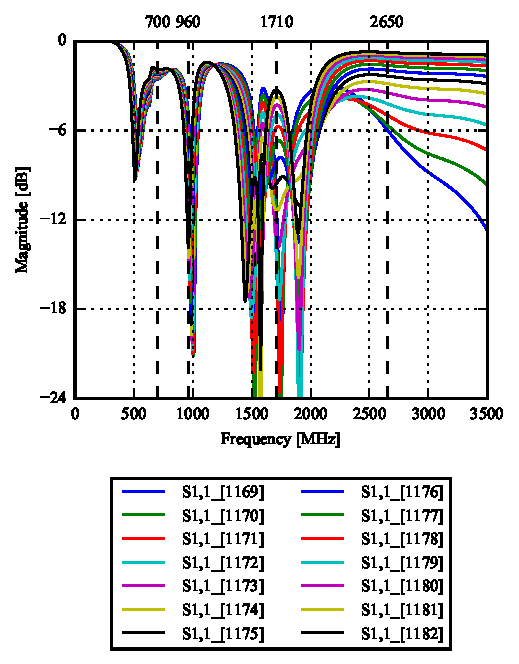
\includegraphics{img/tech_sol/monopole/play_mode/s11}
      \caption{$S_{11}$, sweeping $C_1$ and fixing $C_2$.}
    \end{subfigure}
    \hfill
    \begin{subfigure}[b]{0.49\linewidth}
        \centering
        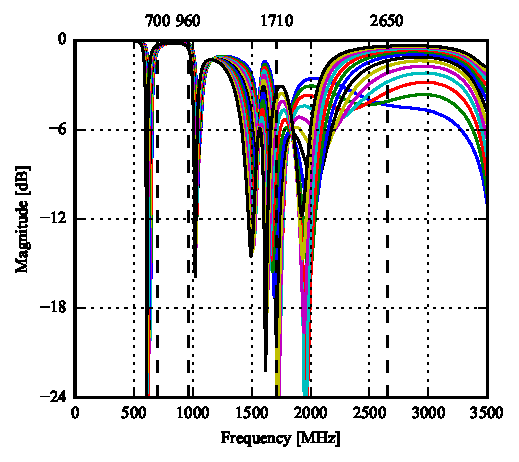
\includegraphics{img/tech_sol/monopole/play_mode/s22}
        \caption{$S_{22}$, sweeping $C_2$ and fixing $C_1$.}
    \end{subfigure}
~
    \begin{subfigure}[b]{0.49\linewidth}
        \centering
        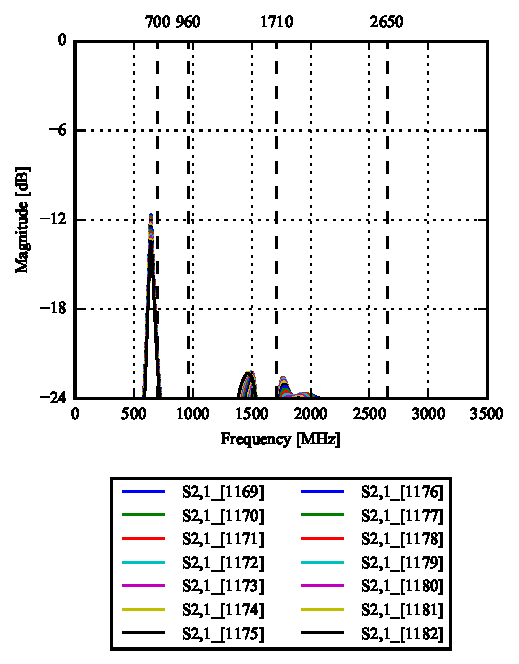
\includegraphics{img/tech_sol/monopole/play_mode/s21_s11}
        \caption{$S_{21}$, sweeping $C_1$ and fixing $C_2$.}
    \end{subfigure}
    \hfill
    \begin{subfigure}[b]{0.49\linewidth}
        \centering
        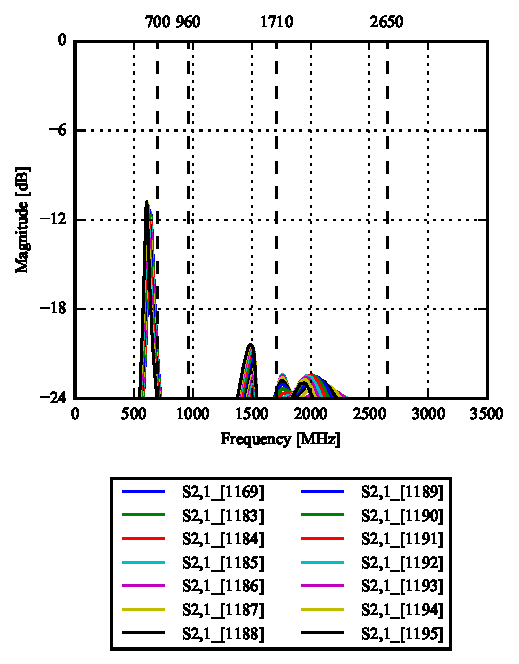
\includegraphics{img/tech_sol/monopole/play_mode/s21_s22}
        \caption{$S_{21}$, sweeping $C_2$ and fixing $C_1$.}
    \end{subfigure}
    \caption{S-parameter sweep in play mode for tuning the shunt capacitor of each antenna, $C_1$ and $C_2$ for port 1 and 2, respectively. Port 1 is the top antenna and port 2 is the side antenna.}
    \label{fig:sparam_mono_play_mode}
\end{figure}

% Correlation
\begin{figure}[htbp]
    \centering
    \begin{subfigure}{0.49\linewidth}
        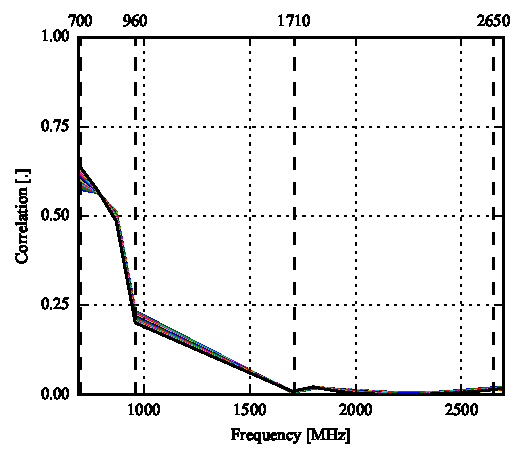
\includegraphics{img/tech_sol/monopole/play_mode/s11_corr}
        \caption{Sweeping $C_1$ and fixing $C_2$.}
    \end{subfigure}
    \hfill
    \begin{subfigure}{0.49\linewidth}
        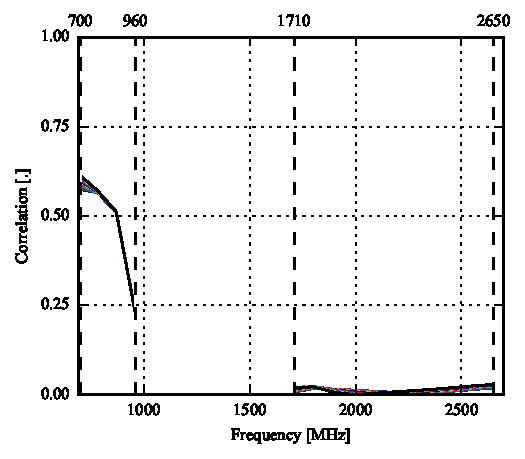
\includegraphics{img/tech_sol/monopole/play_mode/s22_corr}
        \caption{Sweeping $C_2$ and fixing $C_1$.}
    \end{subfigure}
    \caption{Monopole antenna in play mode. Correlation between antennas when sweeping tuning capacitors. Here, $C_1$ and $C_2$ are the tuning capacitor for the top and side antenna, respectively.}
    \label{fig:corr_sol1_play}
\end{figure}

%Efficiency
\begin{figure}[htbp]
    \centering
    \begin{subfigure}{0.49\linewidth}
        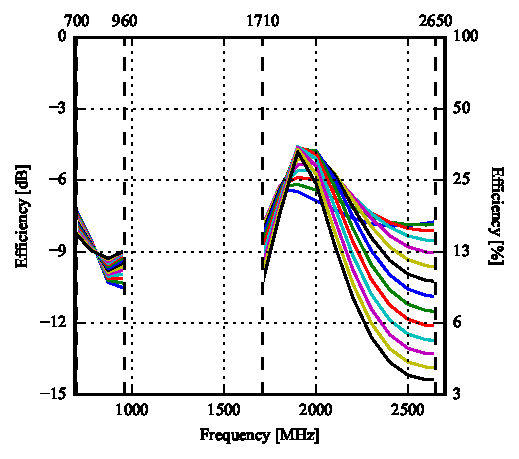
\includegraphics{img/tech_sol/monopole/play_mode/efficiency-ac1-csh1}
        \caption{Sweeping $C_1$ and fixing $C_2$.}
    \end{subfigure}
    \hfill
    \begin{subfigure}{0.49\linewidth}
        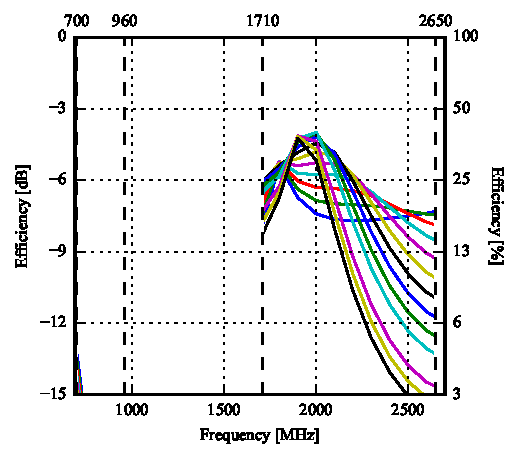
\includegraphics{img/tech_sol/monopole/play_mode/efficiency-ac2-csh2}
        \caption{Sweeping $C_2$ and fixing $C_1$.}
    \end{subfigure}
    \caption{Monopole antenna in play mode. Efficiency for each antenna when sweeping the tunable capacitors. Here, $C_1$ and $C_2$ are the tuning capacitor for the top and side antenna, respectively.}
    \label{fig:eff_sol1_play}
\end{figure}

\FloatBarrier
\subsection{Talk Mode}
%S-parameter
The S-parameter sweeps for the data mode, can be seen on Figure \ref{fig:sparam_mono_talk_mode}. The highest obtainable bandwidth for both antennas is found from the S-parameter sweep and is listed in Table \ref{tab:bw_sol1talk}. The top antenna covers the required bandwidth both in the low band and high band. The side antenna only covers the high band and will need some  additional tuning in the low band. The S-parameter sweeps \ref{fig:sparam_mono_talk_mode} also shows the $S_{21}$ isolation loss. The highest notable isolation loss is within the low band, at \SI{12}{dB} and \SI{8}{dB} both the top and side antenna respectively.

%correlation
The correlation between the top and side antenna can be seen in Figure \ref{fig:corr_sol1_talk}. The correlation is plotted sweeping the tunable capacitors of each antenna, while the other antenna is fixed with a tunable at \SI{0.3}{pF}. The correlation for the top and side exceeds the required correlation limit with 0.15 in the low band from \SI{700}{MHz} to \SI{750}{MHz}.

%Efficiency
The efficiency in talk mode for both antennas, can be seen in Figure \ref{fig:eff_sol1_talk}. The efficiency is plotted for each sweep of the tunable capacitors. Comparing the efficiency in talk mode with the free space efficiency, the talk mode generally decreases over the entire spectrum for both antennas. The different sweep modes of the tunable capacitor shows most significant efficiency drop in the low band. However comparing the individual sweep modes the highest efficiency drop for the top antenna is within the low band at \SI{960}{MHz} and within the high band at \SI{2500}{MHz} for the side antenna. The top antenna efficiency drops more than \SI{-13}{dB} and the side antenna has a maximum drop of \SI{-12}{dB}.
Both antennas has the highest efficiency within the frequency band of \SI{1710}{MHz} to \SI{2300}{MHz} with an efficiency of approximately \SI{-8}{dB} for the top antenna and approximately \SI{-6}{dB} for the side antenna. 
The simulation results are as expected compared to the data mode, as the play mode introduces both head and hand losses.

\begin{figure}[htbp]
    \centering
    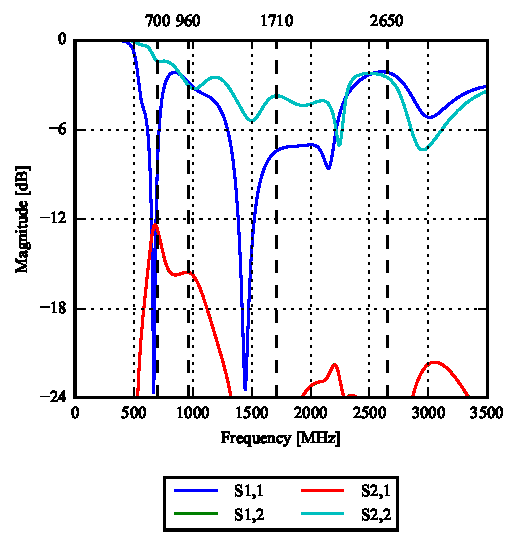
\includegraphics{img/tech_sol/monopole/talk_mode/sparams_talk.pdf}
    \caption{Monopole antenna in talk mode. S-parameters with both tuning capacitors fixed at \SI{0.3}{pF}.}
    \label{fig:mono_talk_sparam_data}
\end{figure}

%bandwidth
\begin{table}[htbp]
    \centering
    \begin{tabular}{|l|l|r|r|r|}
        \hline
        Antenna & Band & Start [MHz] & Stop [MHz] & Bandwidth [MHz] \\
        \hline
        Top     & Low  & 510 & 645  & 135 \\
        Side    & Low  & & & 0    \\
        \hline
        Top     & High & 1092 & 2305  & 1213 \\
        Side    & High & 1335  & 2132 & 797 \\
        \hline
    \end{tabular}
    \caption{Monopole antenna in talk mode. Maximum bandwidth obtained in the low and high band for the top and the side antenna, respectively.}
    \label{tab:bw_sol1talk}
\end{table}

\begin{figure}[htbp]
   \begin{subfigure}[b]{0.49\linewidth}
        \centering
        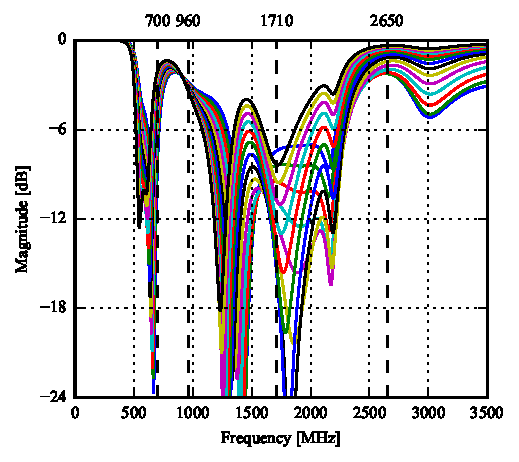
\includegraphics{img/tech_sol/monopole/talk_mode/s11}
        \caption{$S_{11}$, sweeping $C_1$ and fixing $C_2$.}
    \end{subfigure}
    \hfill
    \begin{subfigure}[b]{0.49\linewidth}
        \centering
        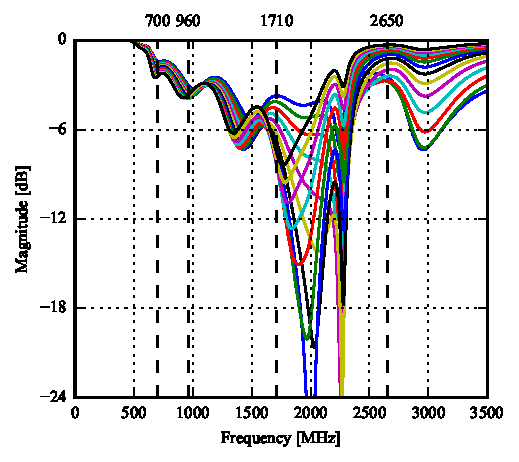
\includegraphics{img/tech_sol/monopole/talk_mode/s22}
        \caption{$S_{22}$, sweeping $C_2$ and fixing $C_1$.}
    \end{subfigure}
~
    \begin{subfigure}[b]{0.49\linewidth}
        \centering
        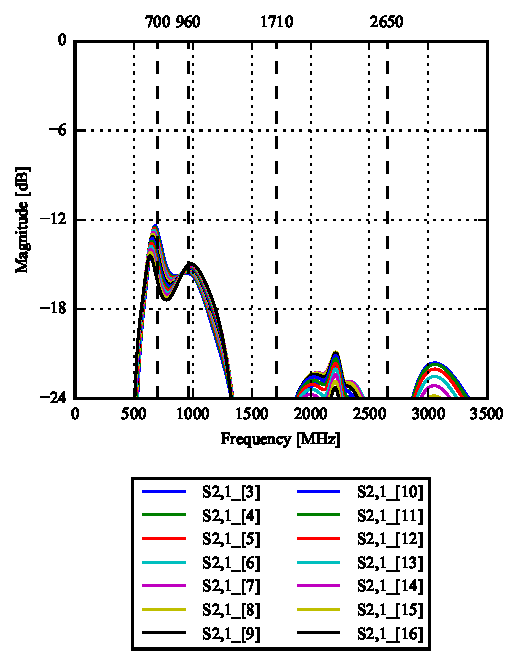
\includegraphics{img/tech_sol/monopole/talk_mode/s21_s11}
        \caption{$S_{21}$, sweeping $C_1$ and fixing $C_2$.}
    \end{subfigure}
    \hfill
    \begin{subfigure}[b]{0.49\linewidth}
        \centering
        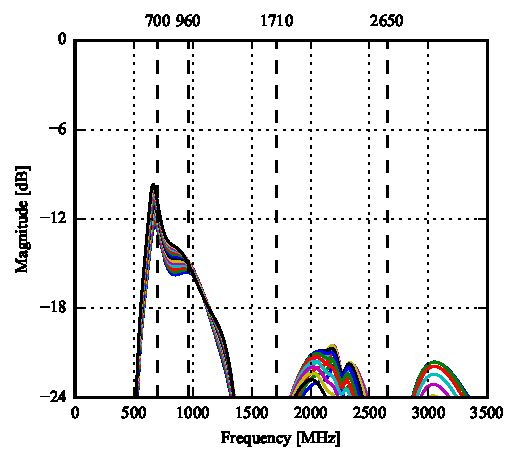
\includegraphics{img/tech_sol/monopole/talk_mode/s21_s22}
        \caption{$S_{21}$, sweeping $C_1$ and fixing $C_2$.}
    \end{subfigure}
    \caption{S-parameter sweep in talk mode for tuning the shunt capacitor of each antenna, $C_1$ and $C_2$ for port 1 and 2, respectively. Port 1 is the top antenna and port 2 is the side antenna.}
    \label{fig:sparam_mono_talk_mode}
\end{figure}
% Correlation
\begin{figure}[htbp]
    \centering
    \begin{subfigure}{0.49\linewidth}
        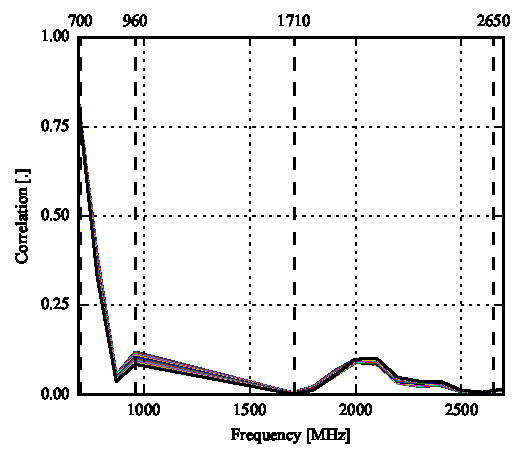
\includegraphics{img/tech_sol/monopole/talk_mode/s11_corr}
        \caption{Sweeping $C_1$ and fixing $C_2$.}
    \end{subfigure}
    \hfill
    \begin{subfigure}{0.49\linewidth}
        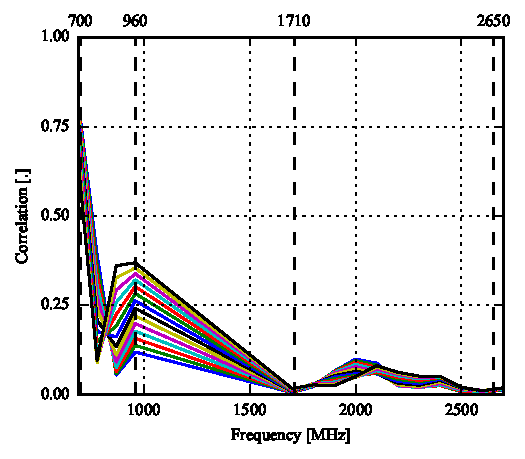
\includegraphics{img/tech_sol/monopole/talk_mode/s22_corr}
        \caption{Sweeping $C_2$ and fixing $C_1$.}
    \end{subfigure}
    \caption{Monopole antenna in talk mode. Correlation between antennas when sweeping tuning capacitors. Here, $C_1$ and $C_2$ are the tuning capacitor for the top and side antenna, respectively.}
    \label{fig:corr_sol1_talk}
\end{figure}

\begin{figure}[htbp]
    \centering
    \begin{subfigure}{0.49\linewidth}
        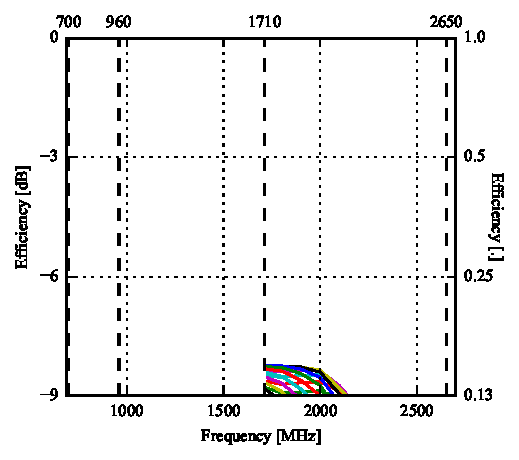
\includegraphics{img/tech_sol/monopole/talk_mode/efficiency-ac1-csh1}
        \caption{Sweeping $C_1$ and fixing $C_2$.}
    \end{subfigure}
    \hfill
    \begin{subfigure}{0.49\linewidth}
        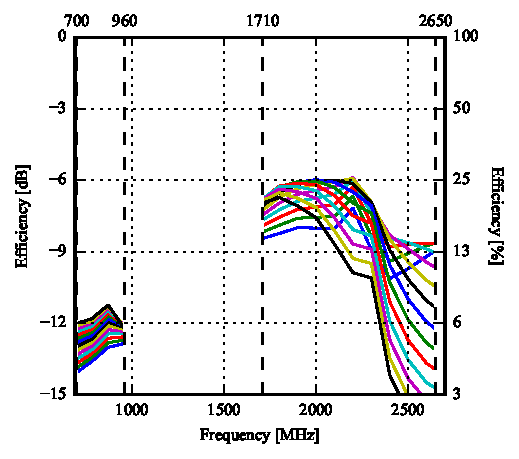
\includegraphics{img/tech_sol/monopole/talk_mode/efficiency-ac2-csh2}
        \caption{Sweeping $C_2$ and fixing $C_1$.}
    \end{subfigure}
    \caption{Monopole antenna in talk mode. Efficiency for each antenna when sweeping the tunable capacitors. Here, $C_1$ and $C_2$ are the tuning capacitor for the top and side antenna, respectively.}
    \label{fig:eff_sol1_talk}
\end{figure}

\FloatBarrier
\subsection{SAR}
The SAR simulation results for both antennas is shown in Figure \ref{fig:sol1_sar}. As seen from the figure, the SAR value for both antennas is within the requirement of \SI{2}{W\per kg}. The top antenna has a maximum SAR value of \SI{1.4}{W\per kg} at \SI{1800}{MHz} and for the side antenna \SI{1.1}{W\per kg} at \SI{1700}{MHz}. Generally the SAR value for both antennas complies with the requirement and is especially low in the low band.
\begin{figure}[htbp]
    \centering
    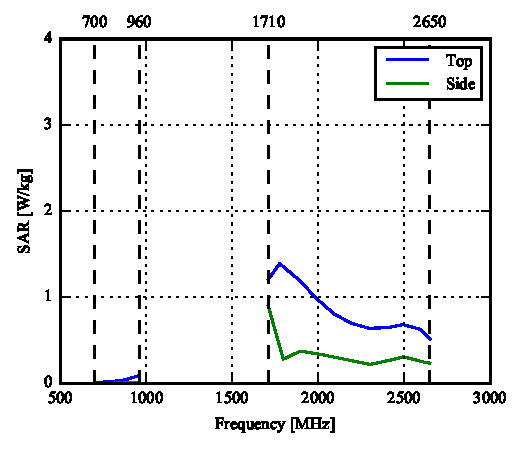
\includegraphics{img/tech_sol/monopole/sar/Top_antenna.pdf}
    \caption{SAR simulation of the monopole antenna.\fixme{new sar plot with screen}}
    \label{fig:sol1_sar}
\end{figure}

